\documentclass[12pt,a4paper,oneside]{book} 
\usepackage[utf8]{inputenc}
\usepackage[spanish]{babel}
\usepackage{amsmath}
\usepackage{array}
\usepackage{amsfonts}
\usepackage{amssymb}
\usepackage{abstract} % Allows abstract customization
\renewcommand{\abstractnamefont}{\normalfont\bfseries} % Set the "Abstract" text to bold
\renewcommand{\abstracttextfont}{\normalfont\small\itshape} % Set the abstract itself to small italic text


\usepackage{amssymb, amsmath}
\usepackage{graphicx}
\usepackage[left=2.54cm,right=2.54cm,top=2.54cm,bottom=2.54cm]{geometry}

\begin{document}
	
	\thispagestyle{empty} 
	
	\begin{center} 
		\LARGE{UNIVERSIDAD PRIVADA DE TACNA} \\[0.5cm] 
		\Large{FACULTAD DE INGENIERÍA DE SISTEMAS}\\[0.5cm] 
		\large{ ESCUELA PROFESIONAL DE INGENIERÍA SISTEMAS} 
	\end{center}
	
	\begin{figure}[htb]
		\centering 
\includegraphics[width=6cm, height=7cm]{img/uptlogo.jpg}
	\end{figure}
	
	\begin{center} 
			\LARGE{\bf PROYECTO TRABAJO FINAL \newline UNIDAD III }\\ \vspace{.25cm}
		
	\end{center}

	\begin{center} 
		
		\textbf {CURSO}\\ 
		\large CALIDAD Y PRUEBAS DE SOFTWARE Sec. A \\
		
		\textbf {DOCENTE}\\
		\large Mag. Patrick Cuadros Quiroga\\
	
		\textbf {INTEGRANTES}\\
		\large Tarqui Montalico, Risther Jaime - 2017057857 \\
		\large Limache Victorio, V\'ictor Piero - 2017057857 \\
		\large Catari Cabrera Yober Nain - 2017059289 \\
		\large Liendo Velasquez, Joaqu\'in - 2017057857 \\
		\large Callata Flores, Rafael - 2017057857 \\
		\large 	Vargas Cusacani, Posi - 2009034478 \\
		
	\end{center}

	
	
	\begin{center} 
		\Large \textsc{Tacna - Perú} \\
		\Large \textsc{2020 } 
	\end{center}

	\newpage
	
	%%INICIO abstract
	\begin{abstract}

		Los productos de software hacen parte de la actividad diaria de la mayoría de las compañías, debido a que la tecnología está presente en cada uno de sus procesos; es así como las empresas desarrolladoras de software tienen un gran reto en crear productos con confiabilidad y calidad. Aquí es donde entran las herramientas de gestión de pruebas estas nos ayudan a gestionar la información relativa a los casos de prueba, para planificar actividades de testing, para gestionar los informes resultantes después de pasar dichos test, etc. Esto es fundamental para cualquier proyecto.\\
		
		\begin{center}
			
			\textbf{Abstract}
		\end{center}
	
		Software products are part of the daily activity of most companies, because technology is present in each of their processes; This is how software development companies have a great challenge in creating products with reliability and quality. This is where the test management tools come in.They help us to manage the information related to the test cases, to plan testing activities, to manage the resulting reports after passing these tests, etc. This is essential for any project. \\
		
	\end{abstract}
	%%FIN abstract
	
	\newpage
	
	\begin{center} 
		\LARGE{\bf PROYECTO TRABAJO FINAL \newline UNIDAD III }\\ \vspace{.25cm}
	\end{center}
	
	\begin{enumerate}
		\item \textbf{INTRODUCCION} \\
			Las empresas desarrolladoras de software que quieran construir sus productos con calidad, requieren un ´área dedicada a la realización de soporte y pruebas, que verifica la funcionalidad y datos de entrada como de respuesta de las transacciones realizadas a las bases de datos desde la aplicación que se está probando, así se hace necesario contar con una trazabilidad de las consultas realizadas a las bases de datos por el ingeniero de soporte y pruebas asignado. \\
			
			De esta necesidad nace la idea de Sistema de Gestión para la ejecución de consultas en pruebas de productos de software, que permite realizar estas mismas actividades mejorando el rendimiento de la maquina en la que se realizan las pruebas y una auditoria o seguimiento posterior a las sentencias que fueron ejecutadas por el ingeniero de soporte y pruebas para la verificación de datos. Con este nuevo modelo se busca obtener ventajas operacionales como: mejor determinación y utilización de la capacidad disponible de los recursos físicos y humanos con los que cuenta la compañía, generando una asignación de recursos que conlleven a un equilibrio de las cargas de trabajo.\\
			
		\item \textbf{TITULO} \\
			Herramientas de Gestión de Pruebas. \\
		\item \textbf{AUTORES}
			\begin{itemize}
				 \item Tarqui Montalico, Risther Jaime 
				 \item Limache Victorio, V\'ictor Piero 
				 \item Catari Cabrera Yober Nain 
				 \item Liendo Velasquez, Joaqu\'in 
				 \item Callata Flores, Rafael 
			\end{itemize}
		\item \textbf{DESARROLLO}
			\begin{itemize}
				\item \textbf{¿QUÉ SON LAS HERRAMIENTAS DE GESTIÓN DE PRUEBAS?}\\
					Es la herramienta que proporciona soporte a la gestión de pruebas y control de parte del proceso de pruebas. A menudo tiene varias capacidades, tales como gestionar los productos de soporte de pruebas, planificación de pruebas, registro de resultados, seguimiento del proceso, gestión de incidencias y generación de informes de las pruebas.\\
					
				\item \textbf{Función de las herramientas de gestión de pruebas}\\
				
					Las tareas de automatización de pruebas están cada vez más presentes en el mercado para automatización de pruebas de software. Existen una serie de herramientas de automatización, pero es poco probable que una sola herramienta pueda automatizar todas las tareas de prueba. La mayoría de las herramientas se centran en una tarea o grupo de tareas específicas, aunque algunas solo tratan un aspecto de la tarea.\\ 
					
					Las herramientas de prueba se pueden categorizar según las funciones que realicen. Algunas designaciones de funciones típicas para herramientas son:\\
					
						\begin{itemize}
							\item Herramientas de adquisición de datos que adquieren datos para utilizar en las tareas de prueba. Los datos se pueden adquirir mediante la conversión, la extracción, la transformación o la captura de datos existentes, o mediante la generación de guiones de uso o especificaciones suplementarias. \\
							\item Herramientas estáticas de medida que analizan información contenida en los modelos de diseño, el código fuente u otros orígenes fijos. El análisis produce información en el flujo lógico, el flujo de datos o la métrica de calidad, como la complejidad, el mantenimiento o las líneas de código.\\
							\item Herramientas dinámicas de medida que realizan un análisis durante la ejecución del código. Las medidas incluyen la operación de tiempo de ejecución del código, como la memoria, la detección de errores y el rendimiento. \\
							\item Simuladores o controladores que realizan tareas que, por cuestiones de tiempo, gastos o seguridad no están disponibles para las pruebas. \\
							\item Herramientas de gestión de pruebas que ayudan en la planificación, el diseño, la implementación, la ejecución, la evaluación y la gestión de tareas de prueba o productos de trabajo.\\
							
						\end{itemize}
				
				
				\item \textbf{Herramientas para realizar pruebas de software }
					Actualmente el número de herramientas para pruebas de software disponibles, tanto en el mercado como de manera gratuita (herramientas de código abierto), es muy amplio. En el siguiente listado os dejamos algunas de las más importantes.
					\begin{enumerate}
						\item Herramientas Open Source
							\begin{itemize}
								\item Herramientas de gestión de pruebas
								\begin{itemize}
									\item Bugzilla Testopia
									\item FitNesse
									\item qaManager
									\item qaBook
									\item RTH(open sourse)
									\item Salome-tmf
									\item Squash TM
									\item Test Environment Toolkit
									\item TestLink
									\item Testitool
									\item XQual Studio
									\item Radi-testdir
									\item Data Generator
									
								\end{itemize}
								
								\item Herramientas para pruebas funcionales
									\begin{itemize}
										\item Selenium
										\item Soapui
										\item Watir (Pruebas de aplicaciones web en Ruby)
										\item WatiN (Pruebas de aplicaciones web en Net)
										\item Capedit
										\item Canoo WebTest
										\item Solex
										\item mprimatur
										\item SAMIE
										\item ITP
										\item WET
										\item Webinject
										
									\end{itemize}
								\item Herramientas para pruebas de carga y rendimiento 
									\begin{itemize}
										\item FunkLoad
										\item FWPTT load testing
										\item loadUI
										\item jmeter
									\end{itemize}
								\item
								
							\end{itemize}
						\item Herramientas comerciales
							\begin{itemize}
								\item Herramientas de gestión de pruebas 
									\begin{itemize}
										\item HP Quality Center/ALM
										\item QA Complete
										\item qaBook
										\item T-Plan Professional
										\item SMARTS5
										\item QAS.Test Case Studio
										\item PractiTest
										\item SpiraTest
										\item TestLog
										\item ApTest Manager
										\item Zephyr
								
									\end{itemize}
								\item Herramientas para pruebas funcionales
									\begin{itemize}
										\item QuickTest Pro
										\item Rational Robot
										\item Sahi
										\item SoapTest
										\item Test Complete
										\item QA Wizard
										\item Squish
										\item VTest
										\item Internet Macros
										
									\end{itemize}
								\item Herramientas para pruebas de carga y rendimiento 
									\begin{itemize}
										\item HP LoadRunner
										\item LoadStorm
										\item NeoLoad
										\item WebLOAD Professional
										\item Forecast
										\item ANTS Advanced .NET Testing System
										\item Webserver Stress Tool
										\item Load Impact
										
									\end{itemize}
							\end{itemize}
					\end{enumerate}
					
				\item \textbf{¿QUÉ ES AWS CODEPIPELINE?}\\
					Es un servicio de Amazon Web Services que nos ayuda a automatizar los procesos de lanzamiento para obtener actualizaciones rápidas y confiables. AWS Codepipeline compila, prueba e implementa tu código cada vez que hay un cambio, en función a los modelos de proceso de los releases que hagas.\\
					
			\newpage			
						\begin{center}
							\begin{figure}[htb]
								\centering 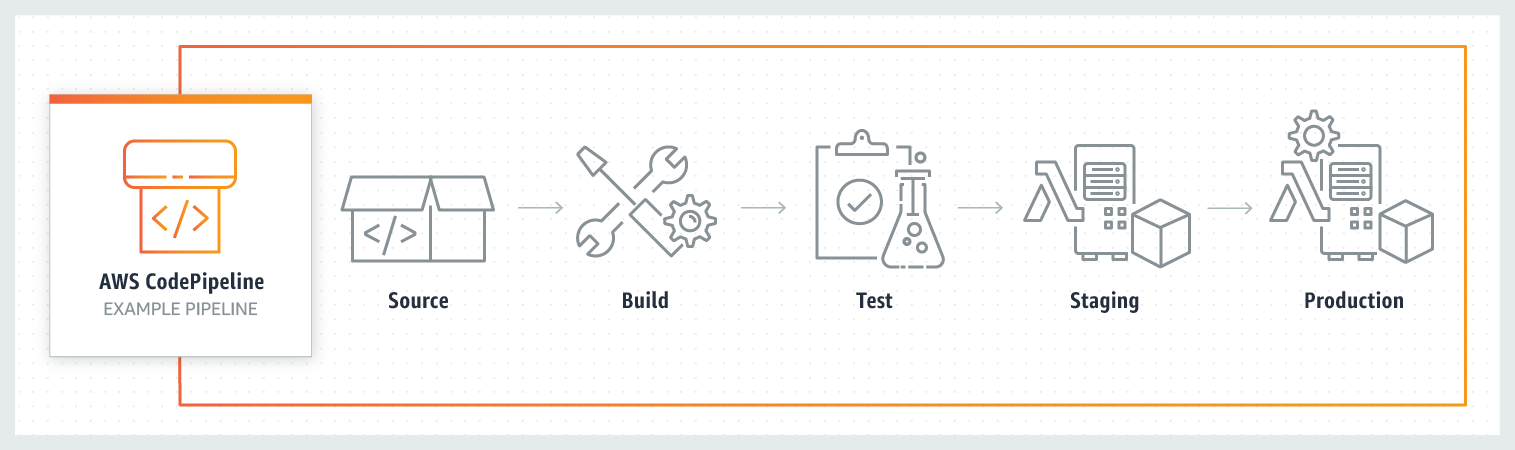
\includegraphics[width=10cm, height=3cm]{img/code.png}
							\end{figure}
						\end{center}
						
					
				\item \textbf{¿QUÉ ES AZURE DEVOPS?}
					Es una plataforma de SaaS (software como servicio) de Microsoft que nos proporciona una cadena de herramientas DevOps de punto a punto para desarrollar e implementar software. También proporciona alojamiento Git privado ilimitado, compilación en la nube para la integración continua, planificación ágil y administración de versiones para la entrega continua a la nube y en las instalaciones. Incluye amplio soporte IDE.\\
					\begin{center}
						\begin{figure}[htb]
							\centering 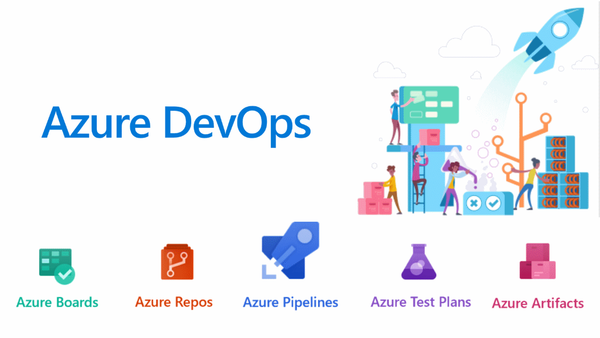
\includegraphics[width=10cm, height=5cm]{img/azure.png}
						\end{figure}
					\end{center}
						
				\item \textbf{COMPARATIVA ENTRE AMBOS: VENTAJAS}
					\begin{center}
						\begin{figure}[htb]
							\centering 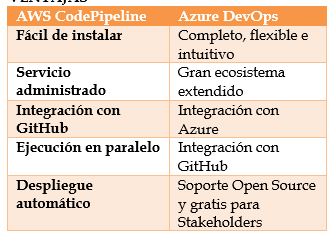
\includegraphics[width=8cm, height=5cm]{img/comparativa1.png}
						\end{figure}
					\end{center}
		 \newpage
				\item \textbf{COMPARATIVA ENTRE AMBOS: DESVENTAJAS}
					\begin{center}
						\begin{figure}[htb]
							\centering 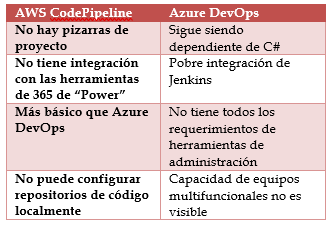
\includegraphics[width=8cm, height=5cm]{img/comparativa2.png}
						\end{figure}
					\end{center}
					
				\item \textbf{COMPAÑIAS QUE USAN ESTAS HERRAMIENTAS:}
					\begin{center}
						\begin{figure}[htb]
							\centering \includegraphics[width=8cm, height=5cm]{img/compañias.png}
						\end{figure}
					\end{center}
				\item \textbf{HERRAMIENTAS QUE PUEDEN SER INTEGRADAS:}
					\begin{center}
						\begin{figure}[htb]
							\centering 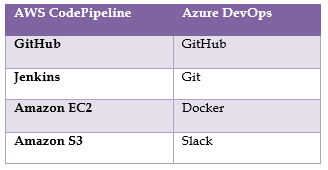
\includegraphics[width=10cm, height=5cm]{img/herramientas.png}
						\end{figure}
					\end{center}
					
				\item \textbf{ALGUNAS BUENAS ALTERNATIVAS A AMBOS:}
						\begin{enumerate}
							\item AWS CodeDeploy
							\item Jenkins
							\item AWS CodeBuild
							\item TeamCity
							\item Bamboo
						\end{enumerate}
			\end{itemize}
		\item \textbf{CONCLUSIONES}
				\begin{enumerate}
					\item CodePipeLine
						\begin{itemize}
							\item CodePipeline es una herramienta de entrega continua e integración continua muy flexible.
							\item Facilita un poco la implementación en el entorno de AWS. Hay una gran disponibilidad de datos no estructurados.
							\item Se usa bastante para gestionar la CI/CD (Integración continua e integración delivery)
							
						\end{itemize}
					\item Azure DevOps
						\begin{itemize}
							\item Es muy fácil de configurar y usar si tiene alguna experiencia con procesos ágiles. 
							\item Las barreras de entrada iniciales son extremadamente bajas, ya que los primeros 5 usuarios pueden aprovechar la herramienta de forma gratuita. Encontré la característica / funcionalidad general más fácil de usar y más accesible que herramientas similares. 
							\item Si ya es un usuario de git, esto se integra directamente con los repositorios de git, lo que facilita la transición. 
							\item La herramienta también está integrada con muchos otros productos de Microsoft, por lo que si tiene una tienda centrada en Microsoft, puede aprovechar el ecosistema más amplio.
							
							
						\end{itemize}
				\end{enumerate}
				
		
		\item \textbf{RECOMENDACIONES}
			Aquí una serie de aspectos a tener en cuenta al momento de elegir una herramienta para la gestión de prueba.
			
			\begin{itemize}
				\item La categoría de defectos
				\item El lenguaje de programación y entorno de desarrollo
				\item El proceso de configuración y gestión de datos de prueba
				\item El control de versiones y CI (Integración Contínua)
				\item Los reportes
				\item Las plataformas compatibles y etiquetado
				
			\end{itemize}
			
		\item \textbf{BIBLIOGRAFIA}
			\begin{itemize}
				
			\item https://stackshare.io/stackups/aws-codepipeline-vs-azure-devops\#:~:text=AWS\%20CodePipeline\%20belongs\%20to\%20\%22Continuous,Workflow\%20Modeling
			
			\item https://www.trustradius.com/products/aws-codepipeline/reviews
			
			\item https://www.trustradius.com/compare-products/aws-codepipeline-vs-azure-devops
			
			\item https://www.infoworld.com/article/3271126/what-is-cicd-continuous-integration-and-continuous-delivery-explained.html
			 
			 \item Fischer G.,” The Software Technology of the 21st Century: From Software Reuse to Collaborative Software Design”
			 
			 \item Pérez B.,” Gestión de las Pruebas Funcionales” 
			 
			\end{itemize}
		
	\end{enumerate}
	
	
	

\end{document}
